\chapter{引言}
\label{cha:intro}


\section{研究背景}

\subsection{知识图谱的发展沿革}

从古至今,信息交流主要依靠语言来进行,人类知识的长期传承也是得益于语言文字这个稳定载体而进行下去的。可以说,从人类早期的莎草纸、羊皮卷、竹简到之后的纸张、书籍,上面的语言文本内容成了知识千年以来突破时空的重要依托。伴随着互联网在二十一世纪的蓬勃发展,信息的传递速度、传递带宽、载体一次性能够传递的信息量都得到了极大的提升,网络文本的存在又将信息传播推向新的高度。信息的增长趋势也从过去线性级别的增长变成了指数级别的增长,这意味着每天都会有成千上万的信息涌入到网络之中,推送到大众面前。这些海量的数据一方面使得信息的来源变得空前丰富,但同时也使得我们对信息的筛选、整理、把握遇到了巨大阻碍。信息爆炸的同时也必然伴随着噪音爆炸,这些海量信息的背后很多是冗余、重复、繁琐,甚至是错误。在这样的环境下,从海量嘈杂的文本之中获取知识是非常不容易的。在这样的背景之下,为了有效地在海量信息之中获取知识、整理知识以及存储知识,知识图谱(Knowledge Graph,KG)的概念被提出,并在学术界和工业界受到了广泛的关注。

知识图谱,某些场景下也被称为知识库(Knowledge Base,KB),是一种将现实世界中人类的知识结构化之后形成的知识系统。在知识图谱中,大量的知识,诸如开放数据库和百科全书中的信息,通常以关系数据集合的形式被表达出来。而在关系数据集合中,基本事实被抽象为实体(Entity),而规则、逻辑、推理等关联性的信息则被抽象为实体间的关系(Relation)。若将实体对应于点,关系对应于边,则这些知识可以进一步以图的形式呈现,从而可以被计算机高效的使用,而这也是研究知识图谱的意义所在。这种将实体和抽象概念结构化成多关系数据集合的模式也是近年来被大力提倡的。可以说,知识图谱使得我们接触到的信息,尤其是知识信息,突破了以往文本字符串中基本的线性构成形式,而以实体与关系构成的网络状形式存在。

目前知识图谱已经作为人工智能领域的一项基础核心技术,被广泛引入到信息检索(Information Retrieval,IR)、问答系统(Question Answering,QA)、推荐系统(Recommender System,RS)等任务上。图谱中优质的结构化知识信息,能够指导我们的智能模型具备更深层的事物理解、更精准的任务查询以及一定程度上的逻辑推理能力,从而在这些知识驱动应用中起到至关重要的作用。可以毫不夸张的说,正是由于这些结构化知识图谱的存在,我们建模实体以及实体之间的关联变的容易起来,让计算机能够理解知识、运用知识甚至于发掘创造知识的想法也逐渐具有了可行性。

\vspace{25pt}
\begin{figure}[!htbp]
\setlength{\abovecaptionskip}{30pt} 
\centering
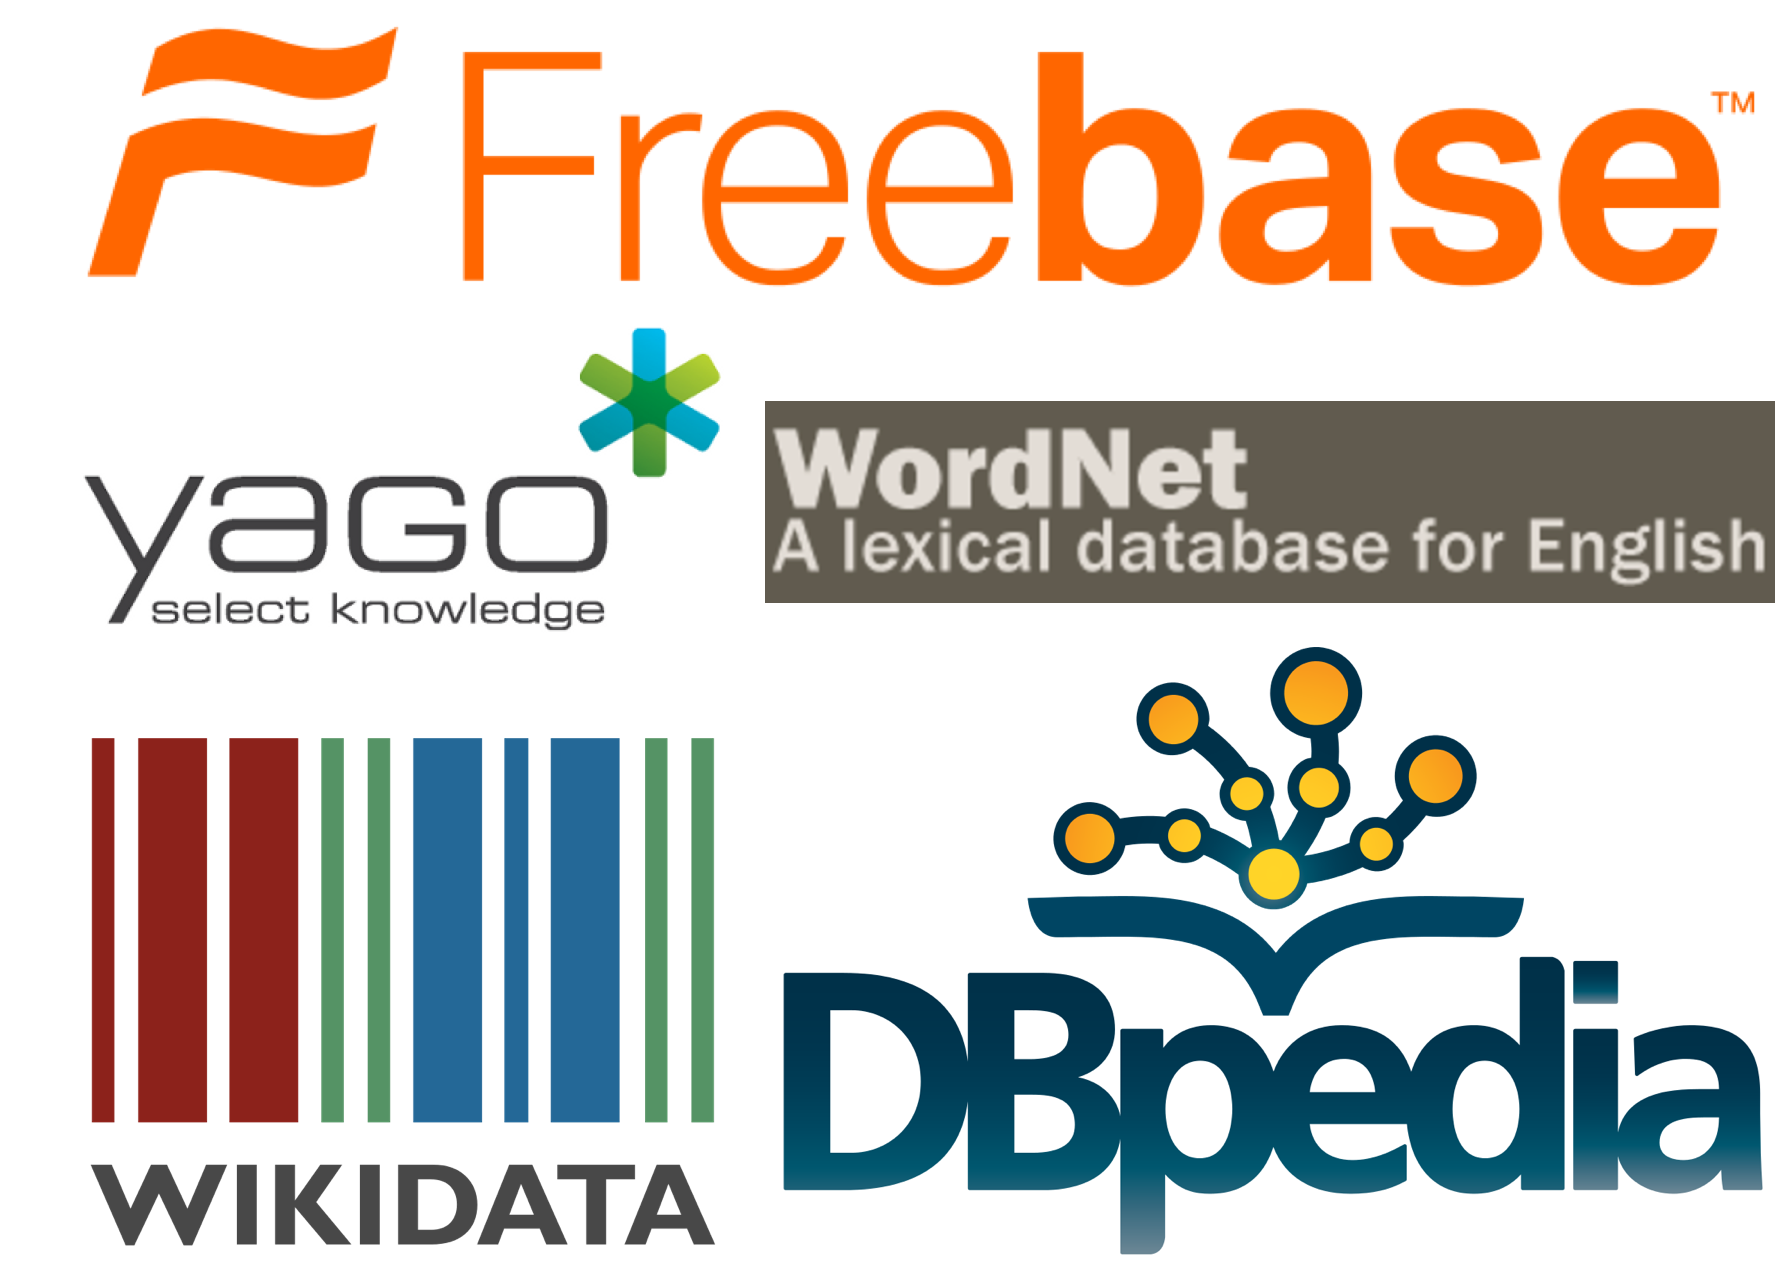
\includegraphics[width=0.8\columnwidth]{figures/ch1/KG_example.png}
\caption{目前公开的大规模知识图谱}
\label{ch1:KG_example}
\end{figure}

伴随着时间的积累以及知识工程工作者长期的工作,结合机器自动标注、专家标注和开放平台编辑校对等多种方法,现在已经构建出一些如图\ref{ch1:KG_example}中展示的高质量大规模知识图谱,包括有 WordNet \cite{miller1995wordnet},YAGO \cite{hoffart2013yago2},DBpedia \cite{auer2007dbpedia},Freebase \cite{bollacker2008freebase},Wikidata \cite{vrandevcic2014wikidata} 以及 Knowledge Vault \cite{dong2014knowledge},并且被投入到部分相关研究场景中。截止到 Freebase 停止更新为止,Freebase 中收集了超过$2$亿个的实体。在其停止维护后,这些信息正在被陆续迁移到 Knowledge Vault 和 Wikidata 中。经过维基社区的过滤和校对,截止目前,Wikidata中也有超过 $2600$ 万个高质量实体存在。与此同时,国内从事互联网领域尤其是和信息检索直接相关的企业也对知识图谱进行了研究投入,百度知心和搜狗知立方作为典型的中文知识图谱被构建出来并被使用到一些智能应用产品中进行知识驱动。

知识图谱将具象事物与抽象概念表示为实体,将实体之间的联系表示为关系,并以( \emph{头实体}, \emph{关系}, \emph{尾实体} )的形式表述知识。例如,“马克·吐温出生于佛罗里达州”在知识图谱中被表述为( \emph{马克·吐温}, \emph{出生于}, \emph{佛罗里达州} );“北京市下辖海淀区”在知识图谱中被表述为( \emph{北京市}, \emph{区划管辖}, \emph{海淀区} )等等。其中\emph{马克·吐温}、\emph{佛罗里达州}、\emph{北京市}、\emph{海淀区}即为实体,而\emph{出生于}、\emph{区划管辖}则是实体间的关系。一般来说,现有公开的知识图谱都是以这样的事实三元组(Triple Fact)形式抽象知识,并采用类似于万维网联盟(W3C)发布采用的资源描述框架(Resource Description Framework, RDF)进行储存。图\ref{ch1:google_kg_example}中展现的就是使用谷歌搜索``北京''时弹出的相关知识图谱。

\vspace{25pt}
\begin{figure}[h]
\setlength{\abovecaptionskip}{30pt} 
% \setlength{\textfloatsep}{60pt} 
\centering
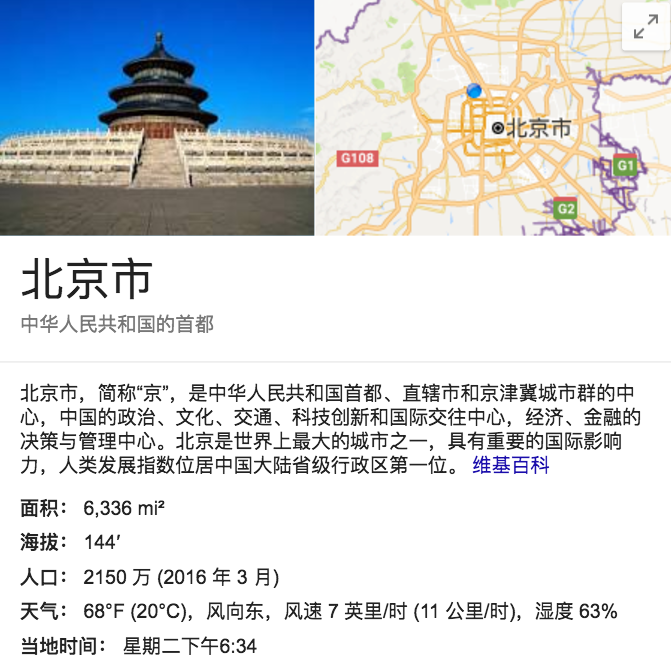
\includegraphics[width=0.6\columnwidth]{figures/ch1/knowledge.png}
\caption{日常搜索中出现的知识图谱信息}
\label{ch1:google_kg_example}
\end{figure}

伴随着上个世纪末互联网的蓬勃发展以及本世纪初信息技术的大量普及,在大量知识被整理进入知识图谱的同时,每天也有大量的知识产生。虽然当前的知识图谱离完善还差的很远,但以结构化形式存在于知识图谱中的知识量之多也是相当惊人的。而伴随着信息的爆炸式增长以及日新月异的变化,这些海量数据如何进行整理、存储、更新以及应用都是巨大的挑战。在这些知识图谱带来的技术诉求之中,很重要的一点就是如何以一个高效的方式进行知识图谱的表示。基于事实三元组集合的形式来表示知识图谱,这可以解决底层数据存储的形式问题,毕竟这与关系数据库的结构十分相似。但这样简单的抽象形式对于理解图谱、应用图谱乃至于依靠知识图谱进行逻辑推演却是远远不够的。想要以高效的形式对知识图谱进行更高层的抽象,并且能够做到利用知识,这其中面临着许多难题:其一,是在计算效率上的问题。知识图谱往往以有向图的形式存在,以点为实体,以边为关系,这样的形式简单明了,却也需要图相关的算法来进行处理。早期基于图结构的图谱表示算法,其计算复杂度通常非常高,以至于在大规模的知识图谱上难以适用。其二,知识图谱中实体和关系的数量十分庞大,却远没有实体数平方级别的事实三元组规模,这意味着知识图谱是稀疏图而非稠密图。与此同时,实体之间的频度也相差很大,满足幂律分布。少部分高频实体和关系涵盖了图谱中多数的事实三元组,其余均是长尾部分。数据的稀疏性以及极端的长尾分布也为模型设计带来了巨大挑战。

\vspace{25pt}
\begin{figure}[h]
\setlength{\abovecaptionskip}{30pt} 
\centering
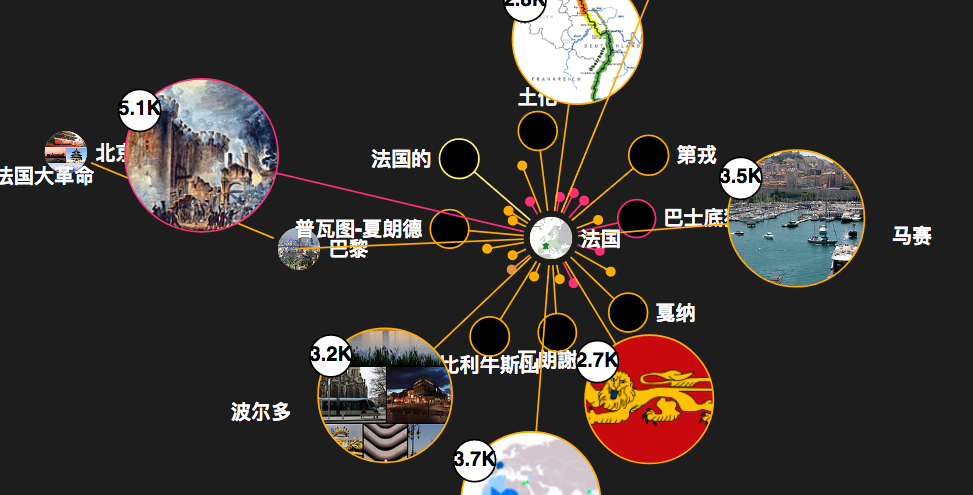
\includegraphics[width=0.9\columnwidth]{figures/ch1/space.png}
\caption{知识图谱 BabelNet 中与实体``法国''空间距离最近的实体}
\label{ch1:space}
\end{figure}

研究与解决知识图谱抽象过程中所面临的计算复杂度与数据稀疏性问题,并将知识图谱表达为计算机可理解使用的模式,就是知识表示学习(Knowledge Representation Learning, KRL)的主要任务。近些年来,受到文本任务中词向量的启发,将图谱进行分布式表示逐渐成为知识表示学习的主流趋势。对于知识图谱来说,所谓的分布式表示(Distributed Representation),其实质就是将图谱中的实体和关系映射到低维度的连续空间中去。在映射空间上,对象之间的距离关系可以直接反映语义关联,比如语义相似的实体,其空间距离一般都十分相近。图\ref{ch1:space}展现的就是空间上与``法国''最相关的实体,数据来源于 BabelNet \footnote{http://babelnet.org/}。因为这个过程实际是将实体与关系的语义信息嵌入到低维度空间上,所以我们通常也将这个过程称为嵌入,得到的向量称为嵌入表示或直接称为嵌入(Embedding)。分布式表示一定程度上解决了之前提到的问题:首先,将知识图谱嵌入到低维度空间上,低维度的空间让实体与关系之间的语义关联计算更加便利,计算量也显著减少。其次,赋予每个实体与关系实数向量的表示形式,并且保持向量之间的空间关系可以用来表示语义关联,很大程度上让知识图谱的分布不再稀疏。最后,以数值形式存在的知识图谱,对于计算机来说比字符形式更容易理解和计算,将其作为其他各个应用模型的输入也变的容易起来。得益于知识图谱表示学习在分布式表示上的有效推进,相关领域的工作也在不断推陈出新,涌现出了一批以知识驱动为内核的模型。

虽然在知识表示学习的研究中已经有大量优秀的模型出现,且在实验数据集合上体现出了模型良好的性能。但是在实验环境中,实验数据集合往往与实际的知识图谱相差甚远,通常只是公开的大规模知识图谱的小子集。通过实际对比可以发现,大规模的知识图谱无论在规模还是在分布上都比实验数据集合更加难以处理,呈现出规模巨大、长尾突出的状态。与此同时,实验过程中模型的设计在突出实验效果考量的同时往往忽略模型自身的复杂程度,其工程实现也难以承受巨大规模的数据处理。另一方面,知识图谱常常会与多源信息进行融合,尤其是与自由文本进行融合。以往的知识图谱与自由文本的融合模型均以串行形式进行融合,这也是很难在极大规模数据量背景下进行训练与处理的模式。本文工作的主要目标,就是立足于现有模型的基础之上,提出一套针对大规模知识图谱的表示学习框架、特征融合框架,在真实的大规模知识图谱上进行训练并能得到优质的嵌入表示。

\subsection{公开的大规模知识图谱}

	\textbf{WordNet}\footnote{http://wordnet.princeton.edu/}是一个以英语词汇与语义为主题的知识图谱,其覆盖范围非常宽广,由美国普林斯顿大学(Princeton University)的科研人员创建。在 WordNet 中,无论是名词、动词、形容词亦或是副词,都会按照其自身语义划分到同义词集中去(Synsets)。整个图谱以同义词集为单位,提供比较精炼的定义和使用示例,形成一个基础的语义单元。同义词集之间,以及同义词集与成员之间,存在一些语言上的关系连接,比如同义词、反义词、蕴涵关系、词元标签以及上下位关系等等。

	\textbf{YAGO}\footnote{http://www.mpi-inf.mpg.de/departments/databases-and-information-systems/research/yago-naga/yago/}是一个综合型知识图谱,由德国马克斯·普朗克研究所(Max Planck Institutes)的科研人员创建。YAGO中的数据,主要来源于对维基百科以及一些网络自由文本的自动抓取。总体上,YAGO拥有超过$1000$万个的实体,以及超过$1.2$亿个实体间的知识事实。2012年之后,YAGO 将 WordNet 的部分语义信息以及 GeoNames 的地理信息融入进来。虽然 YAGO 是自动构建的知识图谱,但对其进行抽样,内部构建的事实准确度高于$95$%。YAGO 被应用在许多实际应用中,尤其是 IBM 的 Watson 智能系统,并且与另一个公开的知识图谱 DBpedia 也有着良好的实体对应。

	\textbf{DBpedia}\footnote{http://wiki.dbpedia.org/}是由德国柏林自由大学(Free University of Berlin)以及莱比锡大学(Leipzig University)的科研人员创建。与 YAGO 类似,DBPedia 也是基于维基百科结构化出的知识图谱,主要功能是强化维基百科的搜寻功能,并将外部的自由文本链接至维基百科。之后 DBpedia 不断发展,现已成为横跨多种语言多种领域的大型综合知识图谱,并且应用在地图整合、多面向搜寻、关系查询、文件分类与标注等多个应用领域上。除上述优点外,DBpedia 还能够自动与维基百科保持同步,且覆盖多种语言。到目前为止,DBpedia 含有超过$125$种语言的知识事实达$30$亿个。

	\textbf{Freebase}\footnote{https://developers.google.com/freebase/}是由自然语言公司 MetaWeb 起初创建的,之后被谷歌(Google)收购,成为谷歌自身知识图谱工程的重要组成部分。与YAGO、DBpedia不同,Freebase是一个庞大的合作知识图谱,主要由社区成员编辑的数据构成,辅助以自动抽取工具。迄今为止,Freebase 是公开的最大规模的知识图谱,包含超过$2$亿个的实体,以及超过$30$亿个的知识事实。Freebase 的数据可以根据创作共用署名许可协议(Creative Commons Attribution License)进行商业和非商业用途,并为程序员提供了极为开放的 API、RDF 备份以及数据库转储,因此成为学术界与工业界图谱研究的主要信息来源。不过在2015年底,谷歌正式宣布了其自身的知识图谱 API 来替代 Freebase 的API,Freebase 也正式关闭,并逐步移入至 Wikidata 中。

	\textbf{Wikidata} \footnote{https://www.wikidata.org/wiki/Wikidata:Main\_Page/} 是维基媒体基金会支持下组织的一个多语言综合知识图谱,主要目的是为维基媒体下的诸多项目(包括维基百科),提供一个概括性的数据框架。在这个框架基础上,大量的文本、图片、影像都被组织在一起。与其他的知识图谱不同,Wikidata 的主要组织形式是文档页面。每个实体均有单独的页面,内部是大量的属性和链接,能够通向其他实体或者维基资源。到目前为止,Wikidata 已有超过$2600$万个实体。Wikidata 有几大显著特点:首先,其本身是一个十分精确的知识图谱,相比自动抓取的知识图谱要精确的多,且近年来在规模上的增长速度也极快。此外,Wikidata 可以统一所有的维基资源,在知识图谱与其他特征进行融合时可以提供大量数据。Wikidata 与所有维基媒体项目一样可以免费使用。 


\section{研究内容}

在前文中,我们点明了知识图谱的重要作用,以及在大规模知识图谱上进行表示学习所面临的诸多问题与挑战。本文工作的主要关注点就是大规模知识图谱表示学习及其相关问题,并对应的在两个方面上提出了改进模型:(1)针对知识表示的基于并行的大规模知识图谱表示学习框架;(2)针对特征融合的基于并行的知识图谱与文本模型联合学习框架。

\subsection{知识表示学习}

第一个是针对知识表示学习的基于并行的大规模知识图谱表示学习框架。知识图谱在信息检索、问答系统等许多应用中起着十分重要的作用,而这些应用程序需要以知识图谱中实体与关系的嵌入表示来作为输入,从而确保模型能够进行高效计算。知识图谱本身也有大量缺损的信息,这个问题同样需要将图谱嵌入到低维度空间中进行表示,并在向量表示的基础上进行图谱推理和填充。出于这两方面的诉求,在以往的工作中,已经出现了一些能够将知识图谱嵌入到连续低维空间中的有效方法。但这些算法出于实现细节问题,虽然在小型知识图谱上得到了效果验证,却并不足以支撑其在大规模知识图谱上进行操作。为了解决大规模知识图谱表示学习的问题,我们提出了一个统一的高效框架,并对已有的一系列经典知识表示模型进行改造,使之融入到我们的体系中进行加速,最终可以在可接受的有限时间内训练出可用的嵌入表示。整体的框架一改以往线性训练模式,而采用多线程带来的并发训练模式。除此以外,我们的框架还在底层上对负样例采样算法进行了优化,而重复的算术运算也得到了合并。为了评估我们框架的高效性和准确性,我们在传统的数据集合上进行了评估。评估结果可以表明,我们的框架可以显著提高知识图谱表示学习的训练效率,且不会对准确率造成影响。框架除了多线程带来的性能收益外,底层的算法操作还可以额外得到近似于十倍的加速。评估之外,我们也对完整的大规模知识图谱Freebase、Wikidata进行了训练,并提供了训练完成后的嵌入表示供研究者直接使用。

\subsection{知识特征融合}

第二个是针对特征融合的基于并行的知识图谱与文本模型联合学习框架。知识图谱的相关资源是十分丰富的,尤其是大量的自由文本。此前,大量的工作在关注知识图谱中事实三元组的结构信息之外,也会将与实体、关系直接相关的文本信息引入到模型内,并将两者特征进行融合。除了知识表示外,文本关系抽取就是一个利用文本信息来丰富知识图谱的任务,其主要目的就是挖掘语义信息来推测实体间的潜在关系。在本文中,我们将知识表示以及文本关系抽取统一为知识获取任务,并提出一个通用的联合学习框架来进行图谱与文本的表示学习。以往的联合学习模型都是以串行连接的方式将图谱模型与文本模型进行联合,而在我们的框架中,我们采用平行的连接方式,期望能够以极快的速度进行训练。在我们的框架设定中,知识图谱和文本模型被统一到一个低维连续空间,同步地学习实体、关系以及文本词语的嵌入表示。在训练过程中,框架通过实体与文本词汇的匹配、关系与文本关系的匹配来分享参数,以达到特征融合的目的。平行交互的联合学习机制可以使得各个部分的模型同时考虑到知识图谱与自由文本的特征信息,从而同时在知识表示和文本关系抽取中取得优异的效果。我们的框架,与现有的进行知识获取的联合学习模型还有一个重大差别,那就是我们的框架十分灵活,图谱部分模型以及文本部分模型均可以被替换为现有的其他经典模型。在实验中,我们也针对性地在知识图谱填充以及关系抽取任务上进行了测试。实验结果表明,在我们联合框架下训练的模型比起单独进行训练的模型,在实验效果上有显著提升。

\subsection{研究要点总结}


	前文我们从宏观角度对我们在知识表示学习、知识特征融合上的工作进行了剖析。在微观研究细节上,我们也将本文开展工作的研究要点及贡献总结如下:

  (1)通过底层实现的优化以及对知识图谱的划分,将以往的图谱模型改造成基于多线程的并发训练模型。在未来,基于多线程的训练模型可以进一步衍生为基于分布式的训练模型,从而能够更高效地对大规模知识图谱进行表示学习。
  
  (2)在多线程进行并发优化之外,我们还提出了基于位移的负样例采样算法来取代原有的负例采样算法。新的采样算法能够在大规模知识图谱的幂率分布下对图中不同的实体和事实赋予不同的注意度,缓解幂率分布带来的长尾影响。与此同时,基于位移的负样例采样方式,可以在训练过程中尽可能的合并算术运算从而进一步进行训练加速。
  
  (3)在知识特征融合方向上,我们采用了平行结合的方式与神经网络文本模型进行融合。相比于过去传统的串行结合方式,基于平行结合的模型能够更快地引入文本信息来丰富图谱内容,并在这个过程中进行特征融合。在平行结合的基础之上,我们提出了一套联合学习框架,使得知识图谱和自由文本能够进行双向的特征融合。在本文框架下训练的图谱和文本模型,经过特征融合之后均有显著效果提升。
  
  (4)本文的工作除了理论阐述与实验证明外,还提供了框架的开源代码并对之前领域内重要的相关工作进行了整理和总结,这些内容的相关信息均已公开发布。这些文档与工具包,为之后需要使用知识图谱的后续研究打好了基础,也能为相关领域的研究工作者提供便利。

\section{论文组织}

为清晰阐述我们的工作,我们罗列了全文的章节安排以及各个章节的内容组织,具体细节如下:

第一章:引言

引言章节,主要立足于一个宏观的角度,整体阐述知识图谱的发展沿革、当前研究界的研究状况,并以此来对论文的研究背景、涉及的重要概念以及选题的实际意义进行诠释。与此同时,引言部分也简要介绍了知识表示学习、知识特征融合的研究内容、研究状态,以及当前研究存在的难点与问题,为之后章节的内容作铺垫。我们也在引言部分给出我们的研究重点与预期工作目标等内容,明确工作中心所在。

第二章:基于并行的大规模知识图谱表示学习框架

在此章节,本文将详细介绍文中提出的基于并行的大规模知识图谱表示学习框架的研究工作,包括研究背景、主要问题与挑战、相关的表示学习模型。这部分内容着重介绍过去几年中被提出的几大类知识表示模型和各自的优劣之处,点明大规模知识图谱表示学习需要解决的核心问题。之后,此章节详细介绍了基于多线程的并行框架与算法原理,实验设置和实验结果分析等。全章通过统一的数学形式将多种知识图谱表示模型高度抽象,统一适配到我们的框架中,并在知识图谱补齐的链接预测任务上进行了评测与实验结果分析,也细节观察了不同线程设置下加速性能的变化以及底层优化所带来的加速提升效果。

第三章:基于并行的知识图谱与文本模型联合学习框架

在此章节,本文将详细介绍文中提出的基于并行的知识图谱与文本模型联合学习框架的研究工作,包括研究背景、主要问题与挑战、相关的联合学习模型。这部分内容着重介绍过去几年中被提出的知识图谱和文本模型的结合方法及相关任务,综述神经网络引入后深度文本模型的发展和联合学习模型的发展。之后,此章节详细介绍了联合框架的模型与算法原理,实验设置和实验结果分析等。全章探索了平行结合方式下的联合学习模型,并在知识图谱补齐、文本关系抽取等任务上进行了评测与实验结果分析,也细节观察了联合学习前后模型在各个任务上的表现变化。

第四章:总结与展望

在总结与展望章节中,我们对本文提出的大规模知识图谱表示学习框架、并行的知识图谱与文本模型联合学习框架进行总结,并分析框架取得的阶段性成果。当然,本文也对自身工作进行了更为深入的分析,罗列了文中提出模型存在的若干问题以及可能的解决办法,同时也对未来可以进行的一系列工作进行了规划与展望。

